\documentclass[12pt,a4paper]{article}
\usepackage[utf8]{inputenc}
\usepackage[english]{babel}
\usepackage{amsmath}
\usepackage{amsfonts}
\usepackage{amssymb}
\usepackage{graphicx}
\author{Guilherme de Sena Brandine \\ Tiago Lobato Gimenes \\ Group: INF582\_08}
\title{Titanic: Machine learning from disaster}

\begin{document}
\maketitle

\section*{Introduction}
The goal of this assignment is to analyse the data from the sinking of the RMS Titanic and, through the usage of techniques of our own choice, attempt to predict, from a set of passengers, which ones have survived. We start out from a training set of 891 passengers whose known information is: The class in which he/she embarked (Pclass), his/her name, sex, age, number of siblings, parents and children, ticket number, fare, cabin and in which port it has embarked. Using the training set, we tried several different approaches to filter which data is relevant for the prediction of survival, and through different combinations of data parsing and supervised learning algorithms, we were able to decide which approach works best.


\section{Data Pre-processing} 
Data pre-processing is an important phase on understanding the problem and consists in filling and parsing the data such that the data is exploitable by data mining algorithms, which work upon generic data. Below, we explain how each column was parsed and/or filled and we give a brief explanation on why we've chosen this method of parsing/filling.
\begin{itemize}
\item \textbf{Passenger ID:} Since this field is already a "numeric" totally filled field and doesn't play an important role on the learning process (The ID does not influence if the person is going to die or not), this field was just copied.

\item \textbf{Passenger Class (Pclass):} Passenger class plays an important role on this problem since, as we can see in figure \ref{class}, people from the third class are more susceptible on dying than those on the first and second classes. Since all of the cells were filled, the only thing made in this column was to subtract one unit of the class because of implementation issues, so the first class became zero, the second became one and so on.

\item \textbf{Name:} We considered that the passenger name does not play an important role on the data mining process, i.e., the passenger name does not influences if the passenger will die or not, so our algorithm does not parse this field, discarding it.

\item \textbf{Sex:} As we can see in figure \ref{sex}, sex plays an important role to the relative number of survivals/deaths and, since this field has the text "male" or "female", we were forced to change to a binary space, where zero was attributed to males and one to females. Since all of the cells of this columns were filled, the simple binary conversion was enough for this feature

\item \textbf{Age:} Since this column isn't complete, we needed to "create" new data in the empty cells. The empty cells were filled with the simple arithmetical mean of all the available ages. The second step was to parse the ages. As we can see in figure \ref{age}, age group plays an important role to the relative number of survivals/deaths. Two approaches were made, one where the algorithm divides in tree age groups as in figure \ref{age} and a second one where nothing was done and the raw age was inserted in the learning algorithm

\item \textbf{Siblings and Spouses (SibSp) and Parents and Children (Parch):} SibSps and Parchs have some cells that are not filled, and our approach consists in filling these with the arithmetical mean of available data. No further discretization is made.

\item \textbf{Ticket, Fare, Cabin and Embarked:} From our studies, these fields do not bring any newer information, so they were discarded in this step.
\end{itemize}

\section{Dimensionality reduction}
Dimensionality reduction is important when many features are used to describe the data, but, in our case, we just have 4 major features, what makes dimensionality reduction not suitable to our case.

\section{Supervised learning algorithms} 

\subsection{Perceptron} 
The perceptron algorithm consists in finding an hyperplane that separates data on two sides, each one corresponding to a side of the binary clustering. It is important to note that the algorithm converges to the correct rotation if the data is linearly separable (ie, if such hyperplane exists), but does not yield satisfying results if the data is scattered around the chosen multidimensional space. 

We used the offline perceptron algorithm, where we repeated the learning process (adjusting the hyperplane rotation for each incorrect prediction of the data) from 1 to 50 times. We first note that there is a 38\% rate of survival in the training data, which is the error rate if we set the initial $w$ to all zeroes. We tried running the perceptron learning algorithm from 1 to 50 repetitions, with eta values equal to 0.0025, 0.25, 0.1, 0.5 and 1. All results were equally effective, yielding an error rate that varies from 27\% to 30\%. This leads to the conclusion that the data is not linearly separable, and hence other approaches should be used. 

\subsection{LDA} 
We then proceeded to the implementation of the Linear Discriminant Analysis (LDA) for two classes, where we search for the projection that minimizes the within-distance of same-class entries and maximizes the distance of both classes' means. By using the code provided in Lab 4, we used the training set to verify the accuracy of the algorithm, which yielded an 86\% accuracy on the training set and a 77\% accuracy on Kaggle. The best accuracy was obtained by using only sex, age, class and siblings as relevant variables. 

\subsection{AdaBoost + Decision trees}
Not being satisfied with the results so far, we've tried a third algorithm, the adaBoost algorithm powered by decision trees. This algorithm is good when trying to separate data that is not separable by hyperplanes. We used the \textit{scikit} library and noticed that the decision tree didn't need to be deep (10) and we didn't need many estimators for the AdaBoost algorithm (10 estimators). With this approach we got 93\% accuracy on the training set and 78\% on Kaggle. The best accuracy was obtained by using only sex, age and class.

\section*{Conclusion} 
Based on our Kaggle submission, we concluded that Perceptron (65\%) is inadequate for such data analysis, LDA (77\%) has a significant prediction success rate, and the best being AdaBoost with 78\%. We researched further to find out that the simple usage of handmade decision trees yields even better results (80\%)  through the correct choice of decision parameters. This is indeed a natural decision based on the aforementioned Data Analysis, where we concluded that sex, class, and age intervals are the most significant factors that influences the survival. A more exhaustive study of data parsing is still possible. For instance, we could also cluster fares to study its influence over the final results, as well as extracting information from names (for example, the Mr, Ms or Miss distinction in names could provide useful information). The relevance of such data can be inferred objectively through formulas such as the Kendall Tau distance (greater absolute values mean bigger correlation) for binary features (sex for instance) or the information gain/chi squared factors.

\section{Attachments}
\begin{figure}[h]
\begin{center}
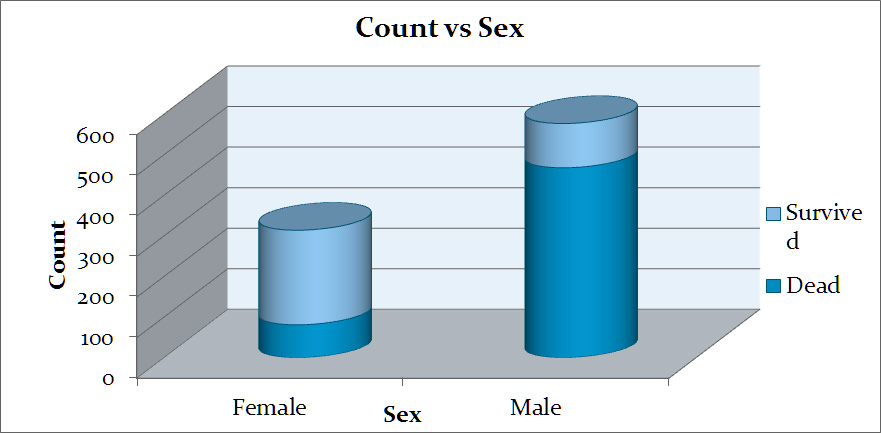
\includegraphics[scale=0.45]{../figures/Sex-vs-Survival.jpg}
\caption{Number of survivals/casualties divided by sex}
\label{sex}
\end{center}
\end{figure}

\begin{figure}
\begin{center}
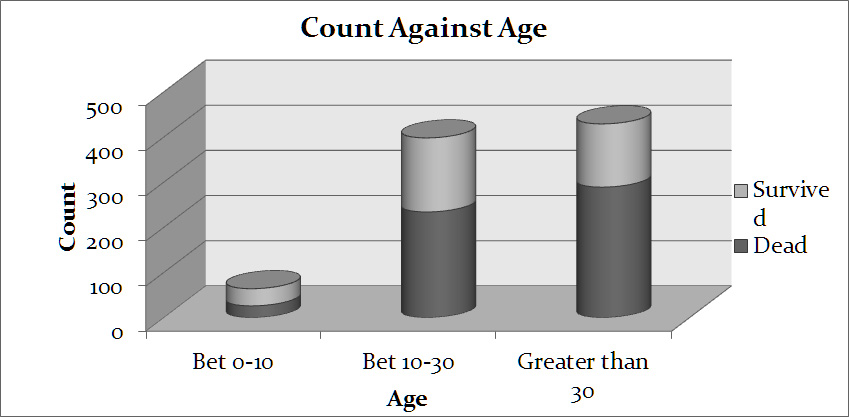
\includegraphics[scale=0.45]{../figures/Age-vs-Survival.jpg}
\caption{Number of survivals/casualties divided by age}
\label{age}
\end{center}
\end{figure}

\begin{figure}
\begin{center}
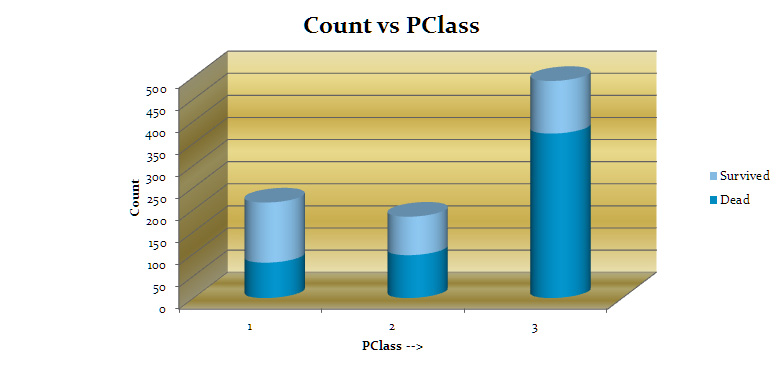
\includegraphics[scale=0.5]{../figures/PClass-vs-Survival.jpg}
\caption{Number of survivals/casualties divided by class}
\label{class}
\end{center}
\end{figure}

\end{document}